\chapter{Implementation}

The following section discuses Web Services, the different plug-ins, and how the product was federated with oneTRANSPORT.

\section{Web Services}
\label{sec:web-services}

The web server (NGINX) was split into different server blocks using virtual host configuration to make a more efficient use of resources. 

There are three server blocks:

\begin{itemize}
  \item Video Streaming Website (portal.sensivision.co)
  \item OM2M User Interface and Web API (om2m.sensivision.co)
  \item OpenMTC Web API (openmtc.sensivision.co)
\end{itemize}

\subsection{VPN}

As mentioned in the design section a VPN was added between the Raspberry Pi and cloud server. Following the tutorial\footnote{https://digitalocean.com/community/tutorials/how-to-set-up-an-openvpn-server-on-ubuntu-16-04} offered by Digital Ocean on setting up OpenVPN on server and client, the team produced the following set-up:

\begin{itemize}
\item \textbf{VPN Server}: 10.8.0.1
\item \textbf{Raspberry Pi 1 IP}: 10.8.0.6
\item \textbf{Raspberry Pi 2 IP}: 10.8.0.12
\end{itemize}

\section{OM2M Sensivision Plug-in}

The \lstinline{om2m.sensivision} plug-in was developed for interacting with the raspberry pi sensors on the MN-CSE and pushing the data to the IN-CSE. It was built based upon the om2m sample light plug-in described in section \ref{light plugin}.

The Sensivision plug-in was created for monitoring each sensor on a Sense HAT add-on board, whether through streams or individual readings.

\subsection{How it Works}

The \lstinline{Activator} class in each plug-in is it’s start point. Inside the class it has the \lstinline{public void start(BundleContext context) throws Exception} method which is called each time a plug-in starts up.

It first registers an IPE Service which, in this case, creates an interface from the Raspberry Pi to the oneM2M standard. The next step then involves ‘discovering’ any CSEs which may be connected to the Raspberry Pi. A CSE is an entity which represents a set of functions of which other entities (AEs, CSEs) can call e.g. Data Management, Device Management, M2M Service Subscription Management etc. The IPE uses the CSE to send requests and the CSE (when it receives a request from a third-party) uses the IPE to carry out the request.

\begin{figure}[H]
  \centering
  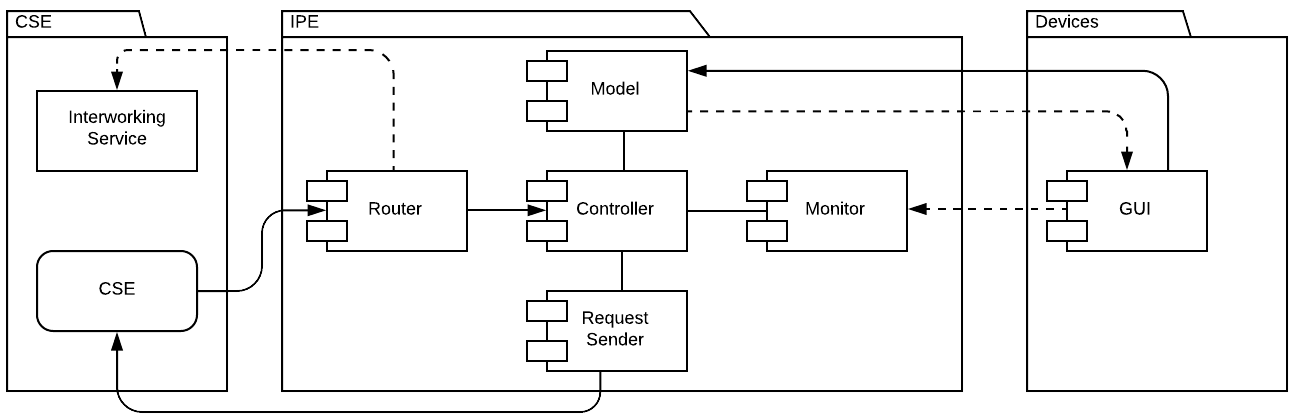
\includegraphics[width=\textwidth]{csemodel.png}
  \caption[OM2M IPE Architecture]{OM2M IPE Architecture \cite{om2mipesample}}
  \label{fig:IPEModel}
\end{figure}

From here, the \lstinline{start} method in the \lstinline{LifeCycleManager} class is called, which creates the application entity representing the Raspberry Pi and within AEs are created representing individual sensors. The AEs representing each sensor have containers within them which can be used to call any of the following 3 methods: \lstinline{GET}, \lstinline{START_STREAM} and \lstinline{END_STREAM}. 

As these containers are created on the MN, containers on the IN are also created to hold the data for each sensor. These containers have a fixed size so when the container becomes full and wants to add another content instance, it removes the oldest and adds the latest (comparable to enqueuing and dequeuing in the queue data structure rather than popping and pushing in a stack). 

The plug-in creates the AEs, containers and content instances is by the \lstinline{RequestSender} class. The sole use of the class is the \lstinline{createResource} method (other methods within the class call the \lstinline{createResource} method and are used for specific type of resources). The method creates a \lstinline{RequestPrimitive} instance (part of the OM2M’s common resource package). Using this instance, it sets multiple variables including the operation type (e.g. create for the creation of the AEs, containers and content instances) using enums, static fields, and additional arguments (the target ID, the resource). This creates the AE on the server once it uses the CSE from the controller to \lstinline{doRequest} passing the \lstinline{RequestPrimitive} as an argument.

The \lstinline{createResource} method returns a \lstinline{ResponsePrimitive} object. With the response the \lstinline{LifeCycleManager} gets the location of where it was created. It uses this as an argument for the IDs of the \lstinline{Descriptor} containers it next creates as well as logging the response from these creations. It then finally creates a content instance in the container. 

The plug-in receives requests via the \lstinline{Router} class. This is set up in the Activator class where it registers the \lstinline{IpeService}. It receives a \lstinline{RequestPrimitive} object from a CSE and from here the router class goes through various validation checks to ensure the request is valid. 

The request is checked for the operation query keyword defined in the \lstinline{SensorConstants} class, its corresponding value will match to one of the following (\lstinline{GET}, \lstinline{START_STREAM} and \lstinline{END_STREAM}). It then checks for the sensor identifier using the sensor query keyword, its corresponding value will match to one of the sensor names also defined in the \lstinline{SensorConstants} class. Using both values, it carries the request. It then returns a \lstinline{ResponsePrimitive}, setting the result of the operation as the content, the content-type a \lstinline{MimeMediaType.OBIX} (XML) and an \lstinline{ResponseStatusCode.OK} response status code.

\subsection{Operations}

Where the Sensivision plug-in differs greatly from the sample lamp plug-in is in the operations it can carry out. It can perform three of the following operations: \lstinline{GET}, \lstinline{START_STREAM} and \lstinline{END_STREAM}. 

All of these operations are managed by the \lstinline{ProcessManager} class whilst the operations themselves are represented by the \lstinline{ProcessRunner} class. The \lstinline{ProcessManager} is used when an operation should either be started or stopped. 

When a \lstinline{ProcessRunner} thread object is initialized it is given three arguments: commands to be executed (an array of Strings), the sensor data is to be collected from (String) and where the data is to be saved (String). The commands are carried out via Python script as there is a python library for retrieving data from a Sense HAT, all scripts differing slightly from one another. Once this object has been called to run, a \lstinline{ProcessBuilder} is used to create a \lstinline{Process} object. The input stream is taken from this object and from that a reader is created to read the incoming data. The data is saved by using the \lstinline{RequestSender} to send a content instance creation request to the IN to be created under the container corresponding to the sensor identifier in the IN.

\begin{itemize}
  \item \textbf{GET}\\
  Retrieve data once from a specified sensor and automatically saves data inside a data container. 
  \item \textbf{START\_STREAM}\\
  Start continuous stream of data from a specified sensor and automatically saves data inside a data container. \lstinline{GET} and \lstinline{START_STREAM} differ in only one extra command string: frequency. If the frequency is not given the \lstinline{Process} will only retrieve data once.
  \item \textbf{END\_STREAM}\\
  Terminates a stream for specified sensor, if one exists.
\end{itemize}

\subsection{OM2M Structure}

Structure of the system starts with the infrastructure node (shown in figure \ref{fig:OM2MInterface}), where all resources registered to it are accessible. Within the node, there is an RemoteCSE, which represents the middle node (labelled \lstinline{mn-pi} in figure \ref{fig:OM2MInterface} and point to the Raspberry Pi). 

\begin{figure}[H]
  \centering
  \frame{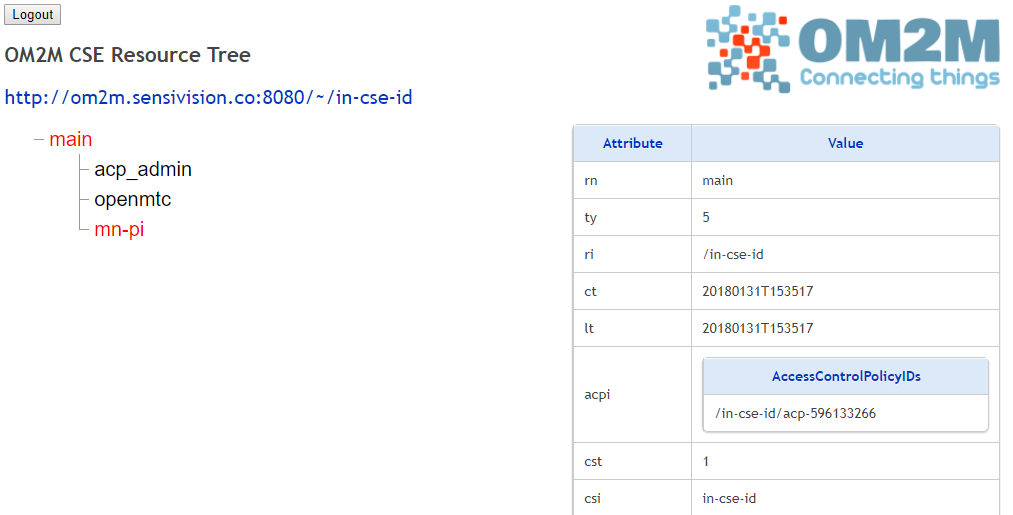
\includegraphics[width=1\linewidth]{om2minterface3.png}}
  \caption{OM2M IN Interface (1)}
  \label{fig:OM2MInterface}
\end{figure}

Figure \ref{fig:OM2MInterface2} shows the resources located under the remote CSE \lstinline{mn-pi}. These are the containers used for storing sensor data with the structure \lstinline{<sensor>_DATA}. This is all located on the IN server. The system was designed this way to avoid data storage on the light Raspberry Pi. 

There is a method whereby the middle node is directly accessible. From figure \ref{fig:OM2MInterface2}, this is the button located at the bottom right (labelled \lstinline{mn-pi-id}). When clicking this button, the IN redirects the user direly to the MN. 

\begin{figure}[H]
  \centering
  \frame{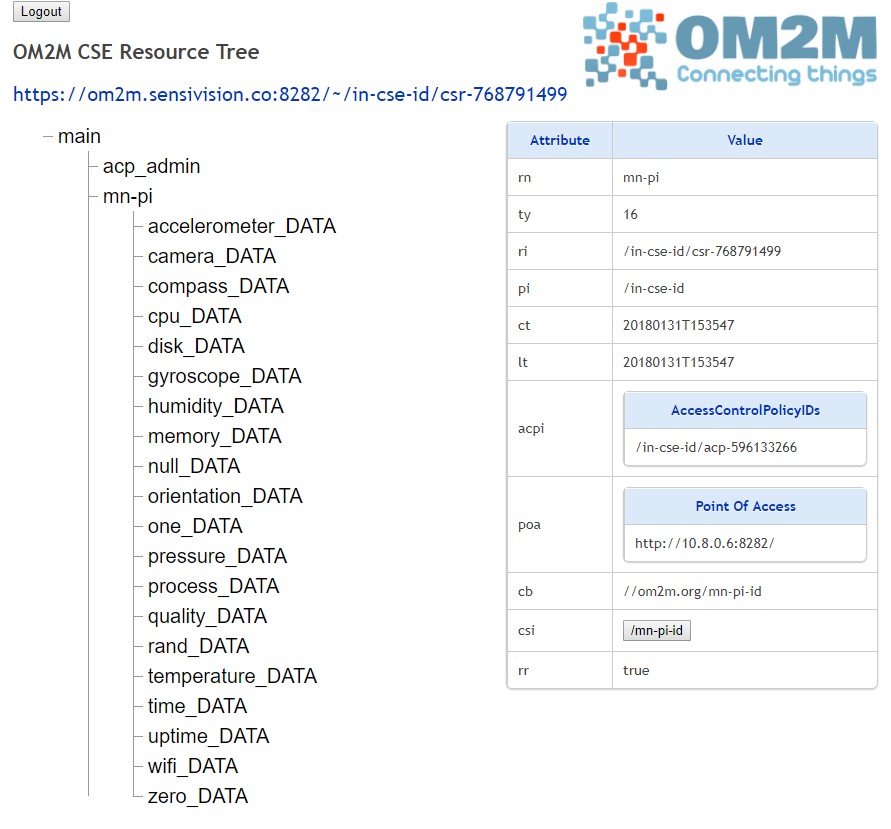
\includegraphics[width=1\linewidth]{INdata}}
  \caption{OM2M IN Interface (2)}
  \label{fig:OM2MInterface2}
\end{figure}

Inside the middle node (figure \ref{fig:OM2MInterface3}) there are multiple application entities, each of which represent a sensor containing the logic for querying and storing the data on the corresponding \lstinline{<sensor>_DATA} container on the IN. Each application entity has a container which has the content instances of the methods: \lstinline{GET}, \lstinline{START_STREAM}, and \lstinline{END_STREAM} shown in red on figure \ref{fig:OM2MInterface4}.

\begin{figure}[H]
  \centering
  \frame{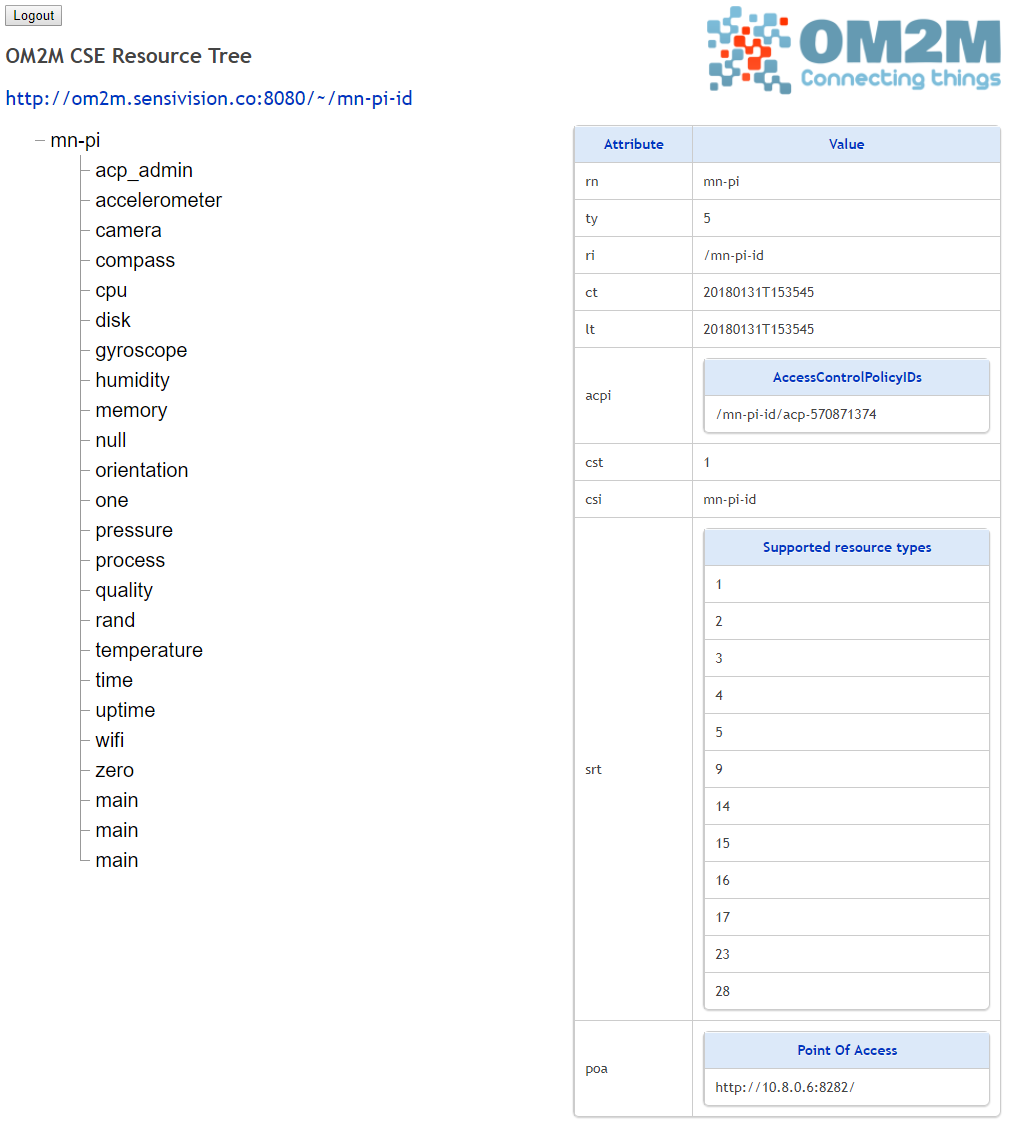
\includegraphics[width=1\linewidth]{om2minterface4}}
  \caption{OM2M IN Interface (3)}
  \label{fig:OM2MInterface3}
\end{figure}

\begin{figure}[H]
  \centering
  \frame{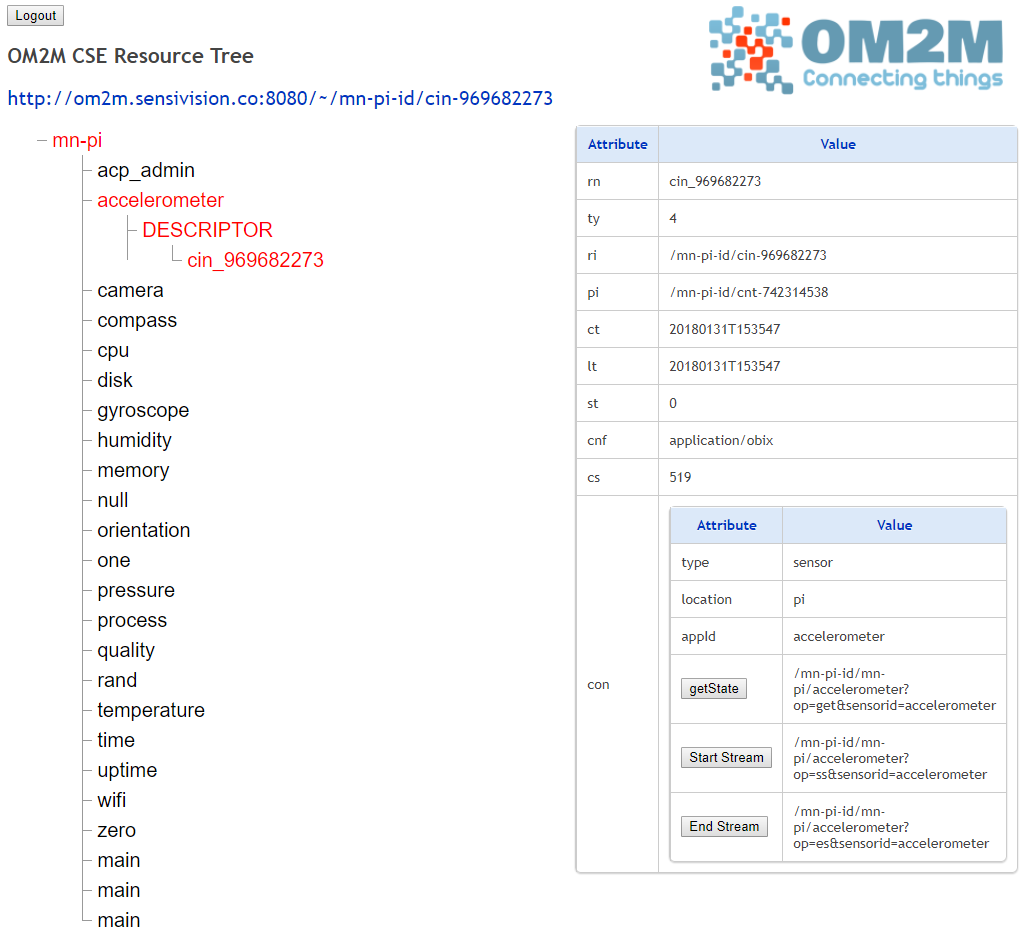
\includegraphics[width=1\linewidth]{om2minterface5}}
  \caption{OM2M IN Interface (4)}
  \label{fig:OM2MInterface4}
\end{figure}

\section{OpenMTC Application}

Due to previously mentioned reasons, the code was ported from OM2M to OpenMTC to allow for further research, and ease of development.

\subsection{Creating Application Entities, Containers and Content}

Application entities are created by passing in the name of the entity to be created (in this case sensor\_data) and the location:\\

\begin{lstlisting}[caption={Creating Application Entities}, label={lst:creating-ae}]
location: '~/in-cse-1/oneM2M'
create_application(AE(resourceName='sensor_data'), location);
\end{lstlisting}

The containers were created by passing in information including the path where the container should be created (inside the application entity) and a container object containing information about the container such as the name (e.g. temperature) and number of content instances that the container can hold (in this case, ten was chosen).\\

\begin{lstlisting}[caption={Creating Containers}, label={lst:creating-containers}]
location = inside the previously created application entity
cont = Container(resourceName='temperature', max=10);
temperature_container = create_container(location, cont); 
\end{lstlisting}

The containers were stored in the Python script as a mapping of the resource name of the container to the container instance, allowing easy access for operations such as adding content instances.\\

\begin{lstlisting}[caption={Creating Content Instances}, label={lst:creating-content-instances}]
registered_sensors['temperature'] = temperature_container;
\end{lstlisting}

To add a content instance to a container, the container to add the data to and the data to add to it, in the form of a JSON, is needed. The JSON contains the current time stamp as well as the value to add (e.g. the current temperature for the temperature sensor). The corresponding container is retrieved via the container mapping described previously.\\

\begin{lstlisting}[caption={Creating Content}, label={lst:creating-content}]
sensor = 'temperature';
data = {
  'timestamp': time.time(),
  'value': value
}
push_content(registered_sensors[sensor], data);
\end{lstlisting}

\subsection{Running the Application}

To run, download the OpenMTC SDK \cite{OpenMTC2017OpenMTC}. Inside the \lstinline{openmtc-gevent} directory there is the \lstinline{run-backend} file and the \lstinline{run-gateway} file. The \lstinline{run-backend} file should be started, followed by the \lstinline{run-gateway}. The IPE created, as described in the previous section, is finally started.

\subsection{Structure}
\label{fig:Structure}

\begin{figure}[H]
\centering
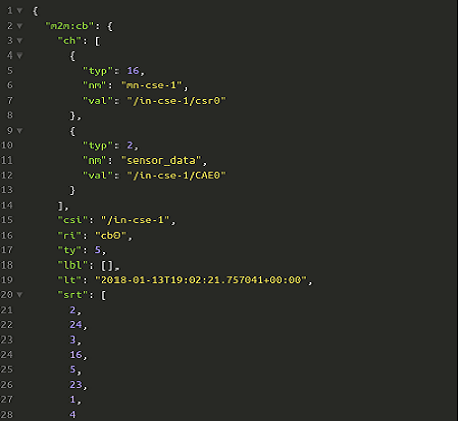
\includegraphics[width=0.5\linewidth]{Type2DataZoom.png}
\caption{Type 2 Data}
\label{fig:Type2Data}
\end{figure}
  
Figure \ref{fig:Type2Data} shows the sensor data application entity created. Line 10 shows the type (type 2 is application entity) and line 11 shows the resource name (sensor\textunderscore data).\\

\begin{figure}[H]
\centering
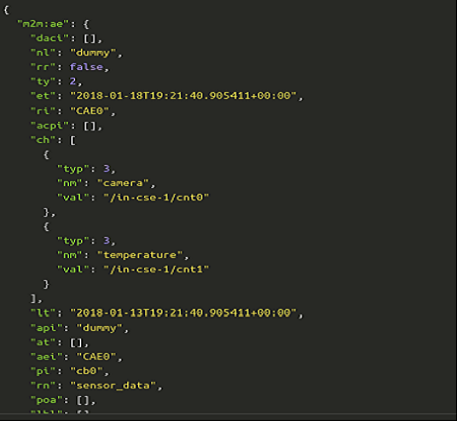
\includegraphics[width=0.5\linewidth]{Type3DataZoom.png}
\caption{Type 3 Data}
\label{fig:Type3Data}
\end{figure}

Figure \ref{fig:Type3Data} shows the containers created. There is both a temperature and camera container of type 3 (representing containers).\\

\begin{figure}[H]
\centering
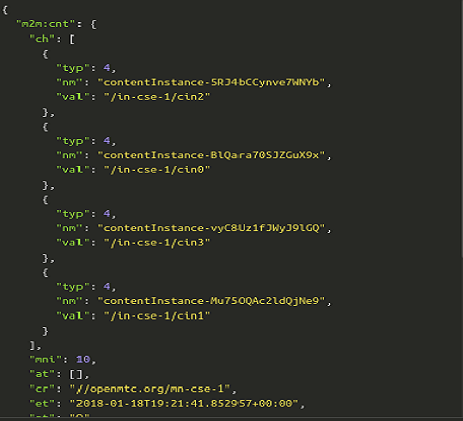
\includegraphics[width=0.5\linewidth]{Type4DataZoom.png}
\caption{Type 4 Data}
\label{fig:Type4Data}
\end{figure}

Figure \ref{fig:Type4Data} shows the inside of the temperature container. Content instances are of type 4 and there are a multitude of type 4 content instances within the temperature container.

\subsection{Rolling Database}

When the maximum number of content instances for a container has been reached, the oldest content instance is removed to make space for the new one. This done so the maximum size of a container may remain fixed and is known as a rolling database. To illustrate this easily, the \lstinline{temperature} containers maximum number of instances will be set to three and the values added will be in the form of strings.

Four content instances, containing the values \lstinline{1}, \lstinline{2}, \lstinline{3}, \lstinline{4}, were pushed into the container of size 3, in that order; what is expected to the see in the temperature container are three content instances where the oldest content instance has the value \lstinline{2}, the second oldest has the value \lstinline{3} and the most recent has the value \lstinline{4}.\\

\begin{lstlisting}[caption={Demonstrating a rolling database}, label={lst:rolling-database-demo}]
push_content(temperature_container, '1');
push_content(temperature_container, '2');
push_content(temperature_container, '3');
push_content(temperature_container, '4');
\end{lstlisting}

\begin{figure}[H]
  \centering
  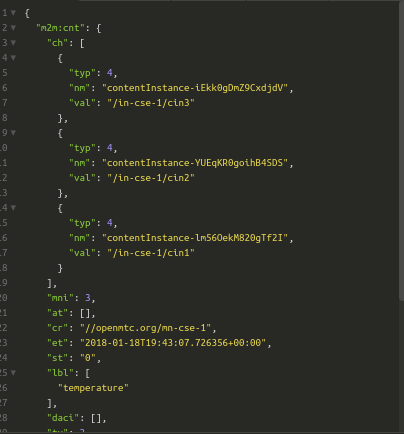
\includegraphics[width=.5\linewidth]{3ContentInstancesZoom.png}
  \caption{Content Instances Inside Temperature Container}
  \label{fig:3ContentInstances}
\end{figure}

There are indeed three content instances inside the temperature container as shown by figure \ref{fig:3ContentInstances} (cin1, cin2 and cin3). To confirm the rolling database, \lstinline{cin1} must contain the value \lstinline{2}, \lstinline{cin2} must contain the value \lstinline{2} and \lstinline{cin3} must contain the value \lstinline{4}.

\subsection{Rolling Database Illustration}
\label{fig:RollingDatabase}

\begin{figure}[H]
\centering
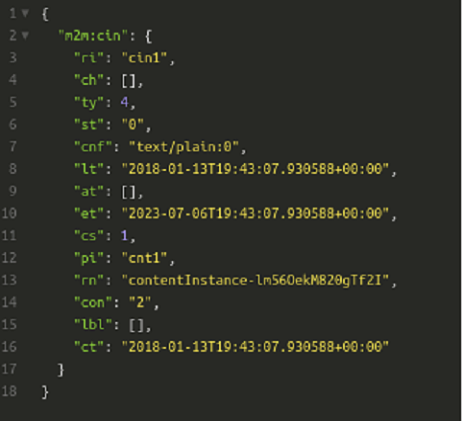
\includegraphics[width=0.5\linewidth]{ContentInstance1Zoom.png}
\caption{Oldest Content Instance}
\label{fig:OldestContentInstance}
\end{figure}

\begin{figure}[H]
\centering
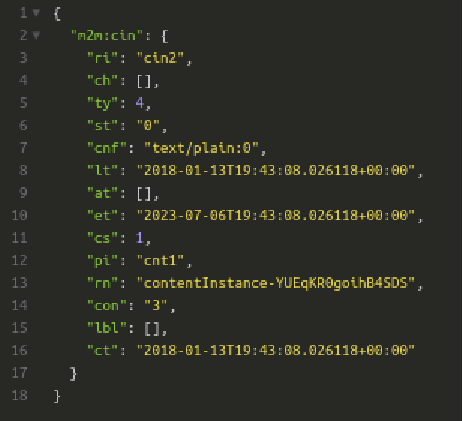
\includegraphics[width=0.5\linewidth]{ContentInstance2Zoom.png}
\caption{Second Content Instance}
\label{fig:SecondContentInstance}
\end{figure}

\begin{figure}[H]
\centering
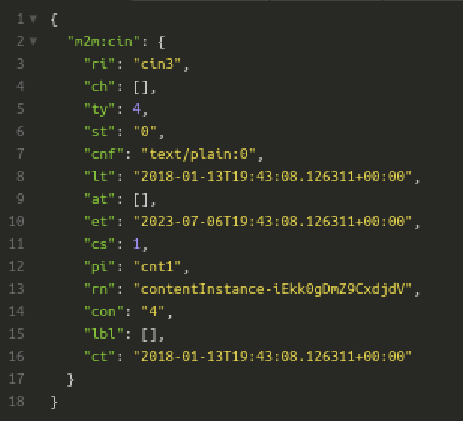
\includegraphics[width=0.5\linewidth]{ContentInstance3Zoom.png}
\caption{Most Recent Content Instance}
\label{fig:MostRecentContentInstance}
\end{figure}

As shown by figure \ref{fig:RollingDatabase}, the values in the content instances (shown by 'con' on line 14) are exactly as predicted. 

\subsection{Camera Streaming}

The following was the process taken to stream the camera data:\\

\begin{lstlisting}[caption={Camera streaming pseudo code}, label={lst:camera-streaming-pseudo-code}]
Repeat until satisfied:
	Capture the current image frame
	Encode in base64 format
	Push data to the server
\end{lstlisting}

Initially camera streaming was done using Eclipse OM2M. This had a terrible frame rate, as a lot of time was required to parse the python code. It was limited to a couple of frames per second at a low 240p resolution. This was improved upon this by disabling logging and reducing the video quality. While it helped, it was not as much as expected. Fortunately, at this point in the project OpenMTC had just been open sourced.

Moving to OpenMTC improved the frame rate. It moved from a few frames per second to close to \textbf{20 frames per second} with a resolution of \textbf{300 $\times$ 300}. This made the stream not only usable but useful, properly demonstrating the powers of OpenMTC. Then, by adjusting JPEG quality, the resolution was raised to 720p, without any major impact on framerate. This proves that oneM2M is can transmit high resolution video, at a good framerate.

\section{Federation}

\subsection{Registering RemoteCSE}
\label{sec:remotecse}

The registration of RemoteCSEs procedures was used by IN-CSE to share data across INs. A successfully registered RemoteCSE is a one-way procedure giving the IN-CSE the ability to use the functions and services hosted on the remote CSE and access the data. This is federation in action.

\begin{figure}[H]
  \centering
  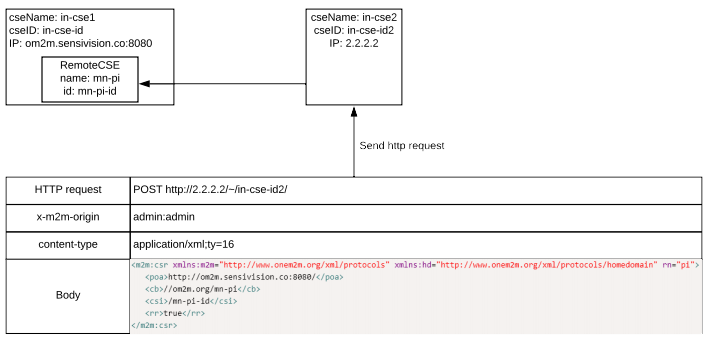
\includegraphics[width=\textwidth]{remotecse}
  \caption[RemoteCSE Registration Procedure]{RemoteCSE registration procedure}
  \label{remotecse}
\end{figure}
  
RemoteCSE registration is done through a single POST request specifying the type of resource to create (type 16). The CSE function take care of establishing communication with the specified host, verifying compatibility and exchanging information. Once this is completed, the IN-CSE with \lstinline{in-cse-id2} has a RemoteCSE resource in its structure named \lstinline{in-cse1} under the root. This will give access to the resources located on \lstinline{in-cse-id}, including the MN-CSE Raspberry Pi with sensor data represented by the \lstinline{mn-pi-id}. 

\subsection{OM2M and OpenMTC Federation}
\label{sec:federation}

The procedure described in section \ref{sec:remotecse} was used to achieve federation between OM2M and OpenMTC. CSE function located on OM2M can access resources in OpenMTC.

The XML shown in figure \ref{fig:federation-post-request} was sent as a HTTP POST request to the OM2M IN.

The fields mentioned in the XML are:

\begin{itemize}
\item \textbf{CSR}: Type of action Create RemoteCSE.
\item \textbf{RN}: Resource name to be displayed by OM2M. 
\item \textbf{POA}: Point of Access of the OpenMTC IN.
\item \textbf{CB}: Callback of the OM2M service provider.
\item \textbf{CSI}: CSE-ID of the OpenMTC IN.
\end{itemize}

\begin{figure}[H]
  \centering
  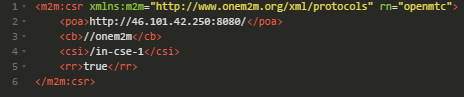
\includegraphics[width=\textwidth]{xml}
  \caption{Federation POST Request}
  \label{fig:federation-post-request}
\end{figure}

This created the remote CSE resource OpenMTC under the root on the OM2M IN that is visible on figure \ref{fig:cseopemtc} highlighted in red.

\begin{figure}[H]
  \centering
  \frame{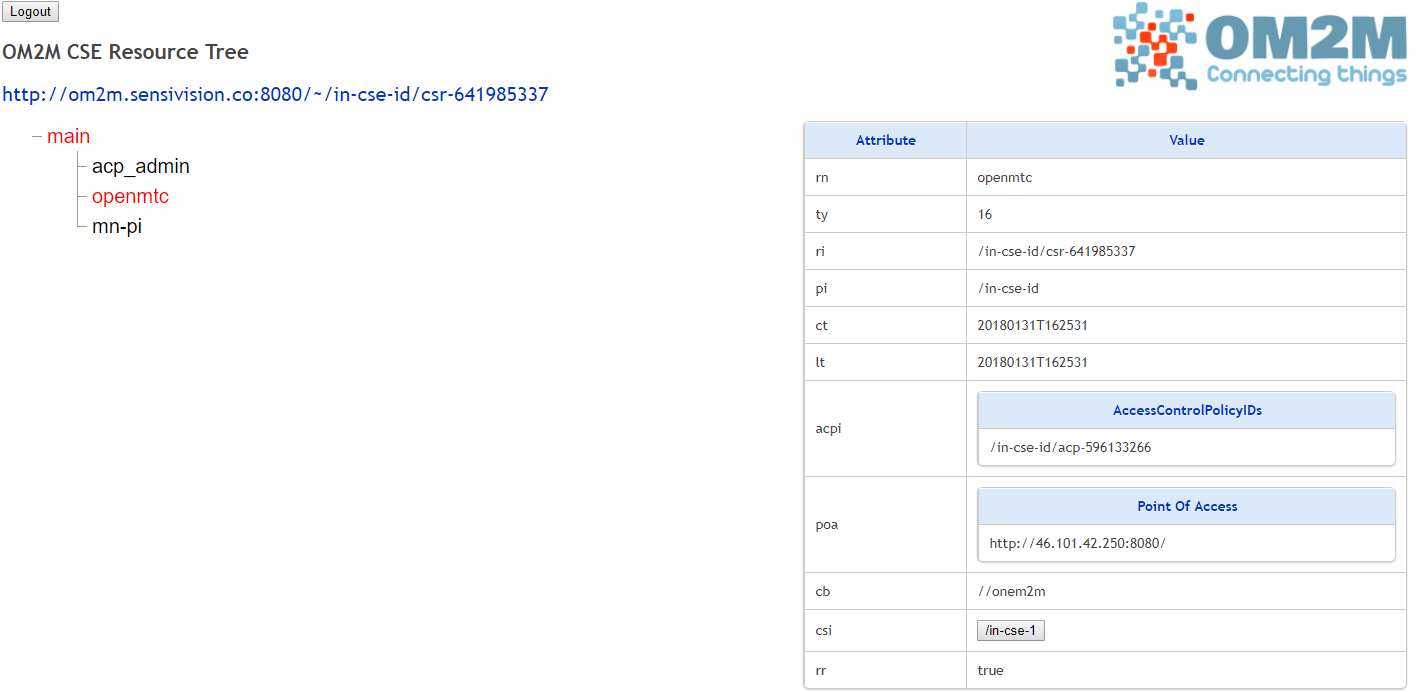
\includegraphics[width=\textwidth]{om2mremotecse}}
  \caption[OpenMTC IN RemoteCSE register on OM2M]{OpenMTC IN RemoteCSE register on OM2M}
  \label{fig:cseopemtc}
\end{figure}

For OM2M's IN to access resources from OpenMTC's IN, the HTTP GET request shown in figure \ref{fig:fed} was sent to the OM2M server. The response, also shown in figure \ref{fig:fed}, displays the resource structure from the OpenMTC IN-CSE.  

\begin{figure}[H]
  \centering
  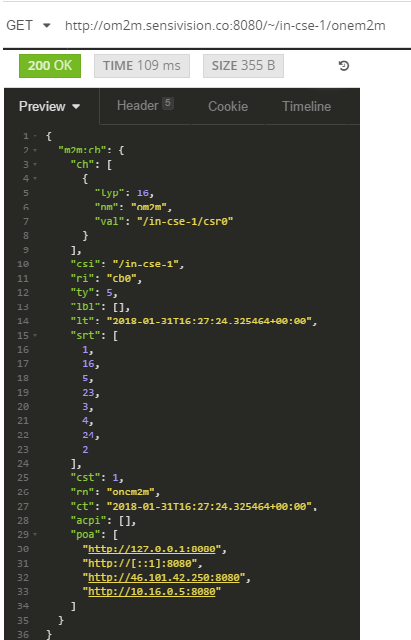
\includegraphics[scale=1]{fed}
  \caption[Federation OM2M to OpenMTC]{Federation OM2M to OpenMTC}
  \label{fig:fed}
\end{figure}

When attempting federating in the opposite direction (OpenMTC to OM2M) the following error appears in the OpenMTC console indicating the unsuccessful communication attempt:\\

\begin{lstlisting}[caption={Failed federation error}, label={lst:federation-error}]
ValueError: 28 is not a valid ResourceType
\end{lstlisting}

The reason for this error will be explained in the evaluation chapter of this report.
       
\subsection{oneTRANSPORT Federation}

The process of demonstrating federation with oneTRANSPORT: 

\begin{itemize}
  \item Run OM2M and OpenMTC IN-CSEs registered to the Raspberry Pi MN-CSEs available publicly. 
  \item Share the Point of Access (PoA) of the infrastructure to the client over email.
  \item The client would attempt the registration of the IN-CSEs through the RemoteCSE procedure, described in section \ref{sec:remotecse}, to try and gain access to the data.
  \item They would reply to the team via email with their findings and issues.
\end{itemize}

The Email Log in the Appendix B - OneTRANSPORT Federation Confirmation shows that the client managed to gain access to the OpenMTC IN-CSE and had access to the content instances in which video stream data was located. 

\clearpage
